%!TEX root = Slic3r-Manual.tex

\section{Scripts de post-traitement} % (fold)
\label{sec:post_processing_scripts}
\index{scripts}
\index{post processing}
\index{post-traitement}

Il peut y avoir des moments o\`u le G-Code g\'en\'er\'e par Slic3r doit \^etre modifi\'e ou modifi\'e apr\`es qu'il ai \'et\'e cr\'e\'e. Pour cette raison, il existe la possibilit\'e d'ex\'ecuter des scripts dans le cadre des derni\`eres \'etapes dans le processus de tranchage\footnote{\url{https://github.com/alexrj/Slic3r/wiki/Writing-post-processing-scripts}}.

\index{Print Settings!Output options!Post-processing scripts}
\index{Param\`etres d'Impression!Param\`etres de sortie!Scripts de post-traitement}
Dans la section \texttt{Output options} (param\`etres de sortie) de l'onglet \texttt{Print Settings} (Param\`etres d'Impression), se trouve l'option \texttt{Post-processing scripts} (Scripts de post-traitement).  Le chemin d'acc\`es absolu de chaque script peut \^etre ajout\'e, s\'epar\'e par des points-virgules. Chaque script doit \^etre reconnu par le syst\`eme h\^ote, et \^etre ex\'ecutable.

\begin{figure}[H]
\centering
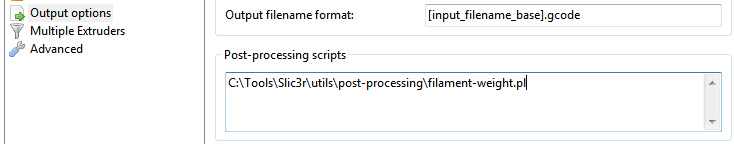
\includegraphics[keepaspectratio=true,width=1\textwidth]{advanced/post_processing_scripts/post_processing_scripts_options.png}
\caption{L'option script de post-traitement.}
\label{fig:post_processing_scripts_options}
\end{figure}

Chaque script sera pass\'e par le chemin absolu du fichier G-code que Slic3r g\'en\`ere. Toutes les options de configuration Slic3r sont mis \`a la disposition des scripts par des variables d'environnement.  Ils commencent tous par \texttt{SLIC3R\_}.  Le script suivant \'ecrira toutes les options Slic3r sur la sortie standard:

\begin{figure}[H]
\small
\begin{verbatim}
        #!/bin/sh
        echo "Post-processing G-code file: $*"
        env | grep ^SLIC3R
\end{verbatim}
\caption{Example de script de post-traitement qui affiche les variables d'environment Slic3r.}
\label{fig:exaple_post_processing_script_env_vars}
\end{figure}

Des exemples de scripts peuvent \^etre trouv\'es dans le d\'ep\^ot GitHub\footnote{\url{https://github.com/alexrj/Slic3r/tree/master/utils/post-processing}}.


le mode "Perl's in-place" (\texttt{perl -i})facilite la modifiction du contenu du fichier G-code, sans avoir \`a copier, modifier, remplacer l'original. L'exemple suivant va simplement afficher le contenu sur la sortie standard:

\begin{figure}[H]
\small
\begin{verbatim}
        #!/usr/bin/perl -i
        use strict;
        use warnings;

        while (<>) {
             # modify $_ here before printing
             print;
        }
\end{verbatim}
\caption{Example de script de post-traitement qui affiche chaque ligne sur la sortie standard.}
\label{fig:exaple_post_processing_script_print_lines}
\end{figure}

% section post_processing_scripts (end)